\chapter{Model Development}




\section{Quad-Rotor Dynamic} \label{sec: quad-model}


Helicopters and quad-rotors are complex flying machines due to their range of maneuverability \cite{Quadrotor_Helicopter_Flight_Dynamics_and_Control, Modelling_and_Control_of_a_Quad_Rotor_Robot}. Traditional helicopters are equipped with tail rotors to counteract the clockwise/anti-clockwise moments due to the motor. However, the \gls{uav} discussed in this report uses a different technique.

Quad-rotors are symmetrical vehicles with four equally sized rotors positioned at the end of their respective mountings. Quad-rotors use  multiple rotors so as to produce greater thrust and increase their maneuverability. Note that adjacent propeller blades are orientated opposite to each other. Thus if one set of rotors is spinning clockwise, then the two adjacent propellers have to spin counter-clockwise so that the torques produced by the propellers balance and cancel out if they all spin at the same rate

\begin{figure}[h]
	\centering
	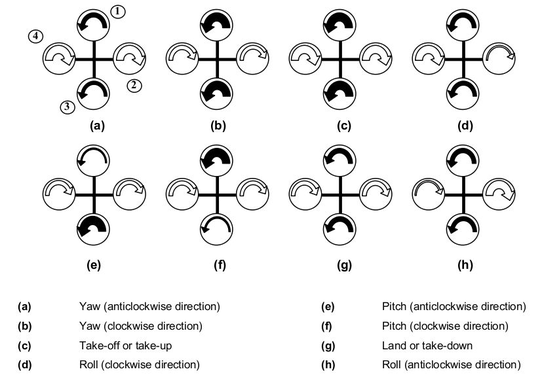
\includegraphics[width =0.7 \paperwidth]{\DocRoot/images/quad-rotor_control}
	\caption{Quad-Rotor Torque Pattern}
	\label{Fig:Quad-Rotor Torque Pattern}
\end{figure}







\subsection{Motor Model}\label{eq: quad rotor model}
For this project a first order linear model of the motor was used to relate motor speed to \gls{pwm}\footnote{ Note it is the duration of the high portion of the signal that sets the speed of the motor, not the percentage of the duty cycle which is high. This is different to traditional \gls{pwm} motor control. }. The first order modeled was used as it was difficult to find accurate values for the inductance and resistance of  the \gls{bldcm} that were used in this project.
\begin{align}
	\dot{\gls{rotationalvelocity}}=\frac{\gls{Motorcontant}\gls{PWMdutycycle}(t) - \gls{rotationalvelocity} }{\gls{timeconstants}}
\end{align}
Note the value for \gls{Motorcontant} was found from the experimental data and is 501.5 $\mathrm{Rad}s^{-2}$.

\subsection{Pitch}
Using Figure \ref{Fig:Quad-Rotor Torque Pattern} as a reference, the pitch of the quad-rotor can be defined using the following equations once one knows the difference in the moments about the pitch-axis.

\begin{equation}
	\tau_{\gls{pitch}} = \sum l \times F =\Delta M =  \gls{trustcoofmotor} \gls{lenghtfromcenterofmass}( \gls{rotationalvelocity}_1 ^2-\gls{rotationalvelocity}_3 ^2)
\end{equation}
Where  \gls{trustcoofmotor} is a constant linking angular acceleration to angular rotation, \gls{lenghtfromcenterofmass} is the distance from the point of rotation to the motors and \gls{rotationalvelocity} is the angular velocity of the motors.Thus, angular acceleration about the pitch axis can be defined as follows:-
\begin{align}
	\ddot{\gls{pitch}} & = \frac{\Delta M}{\gls{interiaofpitch}} =\frac{ \gls{trustcoofmotor} \gls{lenghtfromcenterofmass}( \gls{rotationalvelocity}_1 ^2-\gls{rotationalvelocity}_3 ^2)}{ \gls{interiaofpitch} }
	\label{eq: pitch model}
\end{align}
Where $\omega_1$ \& $\omega_3$ are the speed of motor one and three respectively. 
\subsection{Roll}
Similarly for roll, one can derive the following equation:-
\begin{align}
	\ddot{\gls{roll}} & = \frac{\Delta M}{\gls{interiaofroll}} =\frac{\gls{trustcoofmotor}\gls{lenghtfromcenterofmass}(\gls{rotationalvelocity}_2^2-\gls{rotationalvelocity}_4^2) }{\gls{interiaofroll}}
	\label{eq: roll model}
\end{align}
\subsection{Yaw}
Each of the spinning rotors creates a reaction torque which can cause the quad-rotor to spin about the z-axis which is positioned through the quad-rotor's centre of mass (assuming a uniform frame and equal distancing of the rotor from the centre of mass). Hence, the following equation for yaw can be defined:- 
\begin{align}
	\gls{reactiontorque} = \gls{inertiaofmotor}\dot{\gls{rotationalvelocity}}
\end{align}
The speed of the rotor and the drag coefficient also produce a reaction torque about the yaw axis which can be defined as follows :-
\begin{align}
	\gls{reactiontorquedrag} = \gls{dragcoofmotor} \gls{rotationalvelocity} ^2
\end{align}
Hence the rate of change of yaw is given by the following equation :-
\begin{align}
	\ddot{\gls{yaw}} & =\frac{\sum_{i=1}^{4} \gls{reactiontorque} + \sum_{i=1}^{4} \gls{reactiontorquedrag}  }{\gls{interiaofyaw}}
	\label{eq: yaw undefined}
\end{align}
Filling in for \gls{reactiontorque} and \gls{reactiontorquedrag}  into \eqref{eq: yaw undefined} one gets the following equation :-
\begin{align}
	\ddot{\gls{yaw}}=\frac{\gls{inertiaofmotor}(\dot{\gls{rotationalvelocity} _1}-\dot{\gls{rotationalvelocity} _2}+\dot{\gls{rotationalvelocity} _3}-\dot{\gls{rotationalvelocity}_4})+ \gls{dragcoofmotor} (\gls{rotationalvelocity}_1^2-\gls{rotationalvelocity} _2^2+\gls{rotationalvelocity} _3^2-\gls{rotationalvelocity} _4^2)}{\gls{interiaofyaw}} \label{d2ydt2}
\end{align}
Where, \gls{dragcoofmotor} is the drag coefficient of the propellers and \gls{inertiaofmotor} is the averaged inertia of the motors.  

\subsection{Movement in the Vertical \& Horizontal Directions}

To find the position of the quad-rotor in the vertical direction one can apply Newtons second law to find the following equation :-



\begin{align}
	\ddot{z} & = \left[\frac{\gls{trustcoofmotor}}{\gls{systemmass}}(\cos\gls{pitch} \cos\gls{roll})\sum_{i=1}^{4} \gls{rotationalvelocity} _i^2\right]   -g
\end{align}
Note the sum of the force in the vertical direction must be greater than the weight of the quad-rotor to ensure adequate lift.When the quad-rotor is pitched or rolled it must supply extra thrust to maintain its altitude \cite{identification_and_Control_of_a_Quadrotor_(lund)}.

If it is required to move in the horizontal plane the resultant trust of the quad-rotor has to be resolved as follows by means of Euler Rotations:- \label{Horizontal}
\begin{align}
	\ddot{x} & = \frac{\gls{trustcoofmotor}}{\gls{systemmass}}(\cos\gls{roll}\sin\gls{pitch}\cos\gls{yaw}+ \sin\gls{roll}\sin\gls{yaw} ) \sum_{i=1}^{4} \gls{rotationalvelocity} _i^2 \\
	\ddot{y} & = \frac{\gls{trustcoofmotor}}{\gls{systemmass}}(\cos\gls{roll}\sin\gls{pitch}\sin\gls{yaw} -\sin\gls{roll} \cos\gls{yaw})\sum_{i=1}^{4} \gls{rotationalvelocity} _i^2
\end{align}




\section{Kinematics and Dynamics Equations}

\subsection{Euler Angles} \label{sec: euler angles}
To describe the attitude and position of an object in free space (e.g an aircraft) a reference frame has to be attached to the object and then another can be attached to the earth, after which a relationship between the two coordinate systems can be defined. As the attitude of the device is expressed in the \gls{ned} frame and its angles \& velocity are measured by the \gls{9dof} in the Body Frame. Therefore it is necessary to be able to map from one frame to the other. 

Euler angles \footnote{Note in aviation these form of rotations are commonly refereed to as Tait–Bryan angles and are a sub-set of Euler angles} are not commutative and they must be applied in sequence to get the correct answer \cite[pg. 24]{Stanford_rotation_paper}. In this report the convention  \enquote{\textit{roll,pitch,yaw}}, denoted ($\gls{roll}, \gls{pitch}, \gls{yaw}$), which are rotations about the $(\bf x, y, z)$-axes respectively was adopted. As the accelerometer and gyroscope measurements take place in the Body Frame, the following mapping scheme was introduced so the orientation of the device could be defined in the same frame as the control. A rotation from the \gls{ned} frame to the Body Frame corresponds to a rotation about yaw {\bf R}$(\gls{yaw})^\intercal$, then about pitch {\bf R}$(\gls{pitch})^\intercal$ and finally about roll {\bf R}$(\gls{roll})^\intercal$, these equations are presented fully in \eqref{eq: rotation matrix in z direction1}.     



\begin{align}
	{\bf R}_1(\gls{roll})^\intercal  & \triangleq  \begin{bmatrix}
		1 & 0               & 0              \\
		0 & C_{\gls{roll}}  & S_{\gls{roll}} \\
		0 & -S_{\gls{roll}} & C_{\gls{roll}}
	\end{bmatrix},~
	{\bf R}_2(\gls{pitch})^\intercal & \triangleq  \begin{bmatrix}
		C_{\gls{pitch}} & 0 & -S_{\gls{pitch}} \\
		0               & 1 & 0                \\
		S_{\gls{pitch}} & 0 & C_{\gls{pitch}}
	\end{bmatrix},~
	{\bf R}_3(\gls{yaw})^\intercal   & \triangleq  \begin{bmatrix}
		C_{\gls{yaw}}   & S_{\gls{yaw}} & 0  \\
		- S_{\gls{yaw}} & C_{\gls{yaw}} & 0  \\
		0               & 0             & 1 
	\end{bmatrix}
	\label{eq: rotation matrix in z direction1}
\end{align}


Finally combining these three rotations presented in \eqref{eq: rotation matrix in z direction1} resulted in the following \footnote{For Mathematical ease $\sin(\alpha)$ was simplified to $S_{\alpha}$ and $\cos(\alpha)$ was simplified to $C_{\alpha}$. Note $\alpha$ is a place holder for the angle of interest.}:- 





\begin{equation}
	\gls{rotationmatrix} \triangleq {\bf R}(\gls{roll})^\intercal{\bf R}(\gls{pitch})^\intercal{\bf R}(\gls{yaw})^\intercal  \triangleq  \begin{bmatrix}
		C_{\gls{pitch}}	C_{\gls{yaw}}                                              & C_{\gls{pitch}} S_{\gls{yaw}}                                             & -S_{\gls{pitch}}               \\
		S_{\gls{roll}}S_{\gls{pitch}}C_{\gls{yaw}}  - C_{\gls{roll}}S_{\gls{yaw}} & S_{\gls{roll}}S_{\gls{pitch}}S_{\gls{yaw}}  + C_{\gls{roll}}C_{\gls{yaw}} & C_{\gls{pitch}}S_{\gls{roll}}  \\
		C_{\gls{roll}}S_{\gls{pitch}}C_{\gls{yaw}}  + S_{\gls{roll}}S_{\gls{yaw}} & C_{\gls{roll}}S_{\gls{pitch}}S_{\gls{yaw}}  - S_{\gls{roll}}C_{\gls{yaw}} & C_{\gls{pitch}}C_{\gls{roll}} 
	\end{bmatrix}
	\label{eq: rotation matrix1}
\end{equation}


{\bf where:-} \gls{rotationmatrix} corresponds to the rotation matrix which maps a vector in the \gls{ned} frame to the Body Frame. See Appendix \ref{chap: Rotation Matrix reation} for more information on rotation matrix and Euler Angles



\subsection{Singularities and Gimbal Lock}
Note if \gls{roll}, \gls{pitch} or \gls{yaw} = $\pi/2$ the rotation matrix presented in \eqref{eq: rotation matrix1} losses a degree of freedom. \eqref{eq: gimbel lock example} presents a rotation matrix which has loss a degree of freedom as \gls{pitch} was set equal to $\pi/2$. 

\begin{equation}
	\gls{rotationmatrix} =  \begin{bmatrix}
		0                                                          & 0                                                          & -1 \\
		S_{\gls{roll}}C_{\gls{yaw}}  - C_{\gls{roll}}S_{\gls{yaw}} & S_{\gls{roll}}S_{\gls{yaw}}  + C_{\gls{roll}}C_{\gls{yaw}} & 0  \\
		S_{\gls{roll}}S_{\gls{yaw}}  + C_{\gls{roll}}C_{\gls{yaw}} & C_{\gls{roll}}S_{\gls{yaw}}  - S_{\gls{roll}}C_{\gls{yaw}} & 0
	\end{bmatrix}
	=  \begin{bmatrix}
		0                          & 0                           & -1 \\
		S_{\gls{roll} - \gls{yaw}} & C_{\gls{roll} - \gls{yaw}}  & 0  \\
		C_{\gls{roll} - \gls{yaw}} & -S_{\gls{roll} - \gls{yaw}} & 0
	\end{bmatrix}
	\label{eq: gimbel lock example}
\end{equation}

In aviation this phenomenon is known as Gimbal Lock and corresponds to a reduction in degrees of freedom. As seen from \eqref{eq: gimbel lock example} a change in \gls{roll} and \gls{yaw} has the same effect, thus a degree of uncertainty has been introduced as one notation can represent two very different orientations. This is a problem when using Euler Angles, but as the quad-rotor was limited to $\pm 30^o$ on the \gls{pitch} and \gls{roll} axis this problem was avoided \footnote{Note the problem associated with a loss of freedom due to singularities can be alleviated by using quaternion, but they introduce their own problems as use dimensions to represent a point in free space.}. The limit on the pitch and roll was a result of the lifting power of the motors, once the angle becomes greater than $40 ^o$ the net upwards thrust is less than what is required to maintain the quad-rotor's altitude. 


\section{Inertial Measurement Unit} \label{sec:imu section for relation of stuff}
\subsection{Accelerometer model} \label{sec: acc model}
In order to estimate the attitude\footnote{Attitude are the set of (\gls{roll}, \gls{pitch}, \gls{yaw}) angles in the Body Frame with respect to the \gls{ned} frame.} of the quad-rotor an accelerometer was used to measure the direction of the gravity vector, g , from this the pitch and roll angles can be found. Let g be constant, pointing down along $z_n$ defined in the \gls{ned} frame with an intensity $g_0$ = 9.81 $\mathrm{m~s^{-2}}$ and let
$\bar{\bf a}^B$ denote the accelerometer measurement vector. The definition of $z_n$ can be seen in figure \ref{diag: diagram used to illistrate reference frames}. 

The accelerometer used in this project was an ADXL345, which uses the piezoelectric effect to an create electric signal due to accelerative forces acting on a micro-crystal structure inside the device, knowing this,the following equation was derived:-

\begin{equation}
	\bar{\bf a}^{B} = \gls{rotationmatrix}(g) - a^{B} +\mu_a+ \gls{accbais}  \label{eq:acc full equation1}
\end{equation}
Where: $\bar{\bf a}^{B}$is the sensor output in $\mathrm{m~s^{-2}}$;  g is the gravity vector in the \gls{ned} frame; $a^{B}$ is the acceleration of the quad-rotor; $\mu_a$ is the Gaussian noise component; \gls{accbais} is the constant bias of the accelerometer.


Note when the \gls{9dof} inertial measurement unit is placed at the center of mass \eqref{eq:acc full equation1} can  be shown to simplify to \eqref{eq:acc simplified equation1}. Note  \eqref{eq:acc simplified equation1} doesn't account for the fact that quad-rotor could be in free
fall in a horizontal position. If this occurred the output of the accelerometer would be 0. This could potentially be an issue.

Hence,in order to acquire attitude reads from the accelerometer a model was created that utilized the output vectors of the ADXL345 to estimate the attitude of the quad-rotor. \eqref{eq:acc simplified equation1} was used to estimate the attitude of the quad-rotor.


\begin{equation}
	\begin{bmatrix}
		\gls{ax} \\ \gls{ay} \\\gls{az}
	\end{bmatrix}
	= 
	g
	\begin{bmatrix}
		-S_{\gls{pitch}} \\ C_{\gls{pitch}}S_{\gls{roll}}\\C_{\gls{pitch}}C_{\gls{roll}} 
	\end{bmatrix}
	+
	\begin{bmatrix}
		\mu_{a-x} \\ \mu_{a-y}\\\mu_{a-z}
	\end{bmatrix}
	+
	\begin{bmatrix}
		\gls{accbaisx} \\ \gls{accbaisy}\\\gls{accbaisz}
	\end{bmatrix}
	\label{eq:acc simplified equation1}
\end{equation}





Now assuming that the bias and noise on the accelerometer is zero\footnote{These can be removed in code and by filtering methods respectively. These will be developed later in this report.} the orientation of the quad-rotor in the \gls{ned} frame can be calculated. Hence, \gls{roll} and \gls{pitch} can be defined as follows and can easily be shown to be correct by means of \eqref{eq:acc simplified equation1}:-

\begin{align}
	\begin{split}
		\gls{roll} &= \arctan\left(\frac{\gls{ay}}{\gls{az}}\right)\\
		\gls{pitch} &= \arctan \left(\frac{- \gls{ax}}{\sqrt{\gls{ay}^2+\gls{az}^2}}\right)
		\label{Eq: angles from acc1}
	\end{split}
\end{align}

\subsection{Gyroscope model} \label{sec: gyroscope sec}
A similar model was created for the gyroscope as the angular velocity measured by the gyroscope in the Body Frame doesn't correspond directly to the Euler angle rates $[\dot{\gls{roll}},\dot{\gls{pitch}},\dot{\gls{yaw}}]^\intercal$ . Instead the rate of change of angle can be defined with respect to the \gls{ned} frame as follows:-


\begin{equation}
	\begin{bmatrix}																
		\gls{wx} \\
		\gls{wy} \\
		\gls{wz}
	\end{bmatrix} =
	\begin{bmatrix}																
		1 & 0               & -S_{\gls{pitch}}              \\
		0 & C_{\gls{roll}}  & S_{\gls{roll}}C_{\gls{pitch}} \\
		0 & -S_{\gls{roll}} & C_{\gls{roll}}C_{\gls{pitch}}\end{bmatrix}
	\begin{bmatrix}																
		\dot{\gls{roll} } \\
		\dot{\gls{pitch}} \\
		\dot{\gls{yaw}}\end{bmatrix}
	\label{eq:gyroscope stuf}
\end{equation}

Now taking the in the inverse of \eqref{eq:gyroscope stuf} the following equation can be defined:-
\begin{equation}
	\begin{bmatrix}																
		\dot{\gls{roll} } \\
		\dot{\gls{pitch}} \\
		\dot{\gls{yaw}}
	\end{bmatrix}
	=
	\begin{bmatrix}																
		1 & S_{\gls{roll}}T_{\gls{pitch}}           & C_{\gls{roll}}T_{\gls{pitch}}          \\
		0 & C_{\gls{roll}}                          & -S_{\gls{roll}}                        \\
		0 & \frac{S_{\gls{roll}} }{C_{\gls{pitch}}} & \frac{C_{\gls{roll}}}{C_{\gls{pitch}}}
	\end{bmatrix}
	\begin{bmatrix}																
		\gls{wx} \\
		\gls{wy} \\
		\gls{wz}
	\end{bmatrix}
	\label{Eq: angleur velocity from gyro1}
\end{equation}

\subsection{Digital Compass model}

The magnetometer is a sensor designed to detect the magnetic North direction, written as {\bf  N\textsuperscript I}. By the definition of the reference frame and neglecting  magnetic inclination and magnetic declination, {\bf  N\textsuperscript I} = [0,1,0]\textsuperscript T.

A Honeywell HMC5883L was used in this project. The device works by measuring the change in resistance with a change in the applied magnetic field. The device can measure these change as it is made from strips of permalloy. As the device can measure the change in magnetic field, the orientation of the magnetic field can be estimated using the following:-  
\begin{equation}
	\bar{\bf N}^B = \gls{rotationmatrix}N^I + \mu_m + \gls{gyrobais} \nonumber
\end{equation}
{Where} $\bar{\bf N}^B$ is the sensor measurement which is subject to a Gaussain measurement noise, $\mu_m$, and a bias term, $b_m$.


Now, letting the magnetic field act completely through the $y$ component of \eqref{eq: rotation matrix1} so the quad-rotor will align up with the earths magnetic field along the $y$ axis. Hence, the following relation can be defined:-
\begin{equation}
	\begin{bmatrix}
		{\bf N}_x \\ {\bf  N}_y \\ {\bf  N}_z 
	\end{bmatrix}
	= 
	\begin{bmatrix}
		C_{\gls{pitch}}S_{\gls{yaw}}                                              \\ 
		S_{\gls{roll}}S_{\gls{pitch}}S_{\gls{yaw}}  + C_{\gls{roll}}C_{\gls{yaw}} \\
		C_{\gls{roll}}S_{\gls{pitch}}S_{\gls{yaw}} - S_{\gls{roll}}S_{\gls{yaw}}
	\end{bmatrix}
	+
	\begin{bmatrix}
		\mu_{m-x} \\ \mu_{m-y}\\\mu_{m-z}
	\end{bmatrix}
	+
	\begin{bmatrix}
		\gls{gyrobaisx} \\ \gls{gyrobaisy}\\\gls{gyrobaisz}
	\end{bmatrix}\label{eq: magnetometer read out}
\end{equation}

Thus, if both \gls{pitch} and \gls{roll} are known the compass readings can be compensated by means of the filtered \gls{pitch} and \gls{roll} data. This approach was possible as it was decided to filter the \gls{pitch} and \gls{roll} first and then compensate the \gls{yaw}. An approach similar to the one used on the accelerometer was done when defining \gls{yaw}, that is, the noise and bias were ignored as they can be filtered before \gls{yaw} is calculated. Hence, the following equation was derived so \gls{yaw} could be calculated:-

\begin{equation}
	\gls{yaw} = \arctan\left( \frac{ {\bf N}_x}{C_{\gls{roll}}C_{\gls{pitch}}{\bf N}_y - S_{\gls{roll}}C_{\gls{pitch}}{\bf N}_z - {\bf N}_x }\right)
	\label{eq:yaw com equation}
\end{equation}




\section{GPS Frame Conversion} \label{sec: gps part}
As one of the goals for this project was \gls{gps} navigation by means of way points, which is a method of relating latitude (\gls{latitude}) and longitude (\gls{longitude}) as illustrated in figure \ref{diag: diagram used to illistrate reference frames} was required. Thus, this section will deal with the mapping of \gls{latitude} and \gls{longitude} from a fixed frame attached to the earth (denoted \gls{ecef} to the \gls{ned} frame \cite{crassidis2006sigma}. 


If the quad-rotor required to move a certain distance in the $x, y$ or $z$ direction,this  distance has to be found in the \gls{ecef} frame first. The difference between the current location and the desired location must to be calculated. This difference can be found if the \gls{latitude} and \gls{longitude} of the destination is known and current \gls{latitude} and \gls{longitude} the quad-rotor is known. Once this is known, \eqref{Eq: xyz distance in circle coordinance1} can be used to find $xyz$ displacement in the \gls{ecef} and this is then mapped to the \gls{ned} frame using \eqref{Eq: ecef frame mapping1}. Note a similar approach can be used to control the velocity of the quad-rotor in the \gls{ned} frame.


\begin{align}
	\begin{split}
		N &= \frac{a}{\sqrt{1 - e^2\sin^2\gls{latitude}}}\\
		x&= (N+h)\cos(\gls{latitude})\cos(\gls{longitude})\\
		y &= (N+h)\cos(\gls{latitude})\sin(\gls{longitude})\\
		z &= [N(1-e^2)+h]\sin(\gls{latitude})
	\end{split}
	\label{Eq: xyz distance in circle coordinance1}
\end{align}


{

\begin{description}[itemsep=1mm]
	\item[{\bf Where:-}]
	\item[$h$:] is the height of the quad-rotor from the surface of the planet.
	\item[$a$:] is the equatorial radius of the earth and is equal to 6,378,137~$m$
	\item[$b$:] is the polar radius of the earth and is equal to 6,356,752.3142~$m$
	\item[$f$:] is flatting of the earth and is given by the following:- $f = (a-b)/a$
	\item[$e$:] is the eccentricity of the earth and is defined as follows:- $e= \sqrt{f(2-f) }$
\end{description}
}


In order to find out how far the quad-rotor has to go in order to reach the required position\footnote{And hence also control the quad-rotor} \eqref{Eq: xyz distance in circle coordinance1} has to be mapped using the following:-



\begin{equation}
	\begin{bmatrix}																
		\gls{north} \\
		\gls{east}  \\
		\gls{down}
	\end{bmatrix}
	\triangleq
	\begin{bmatrix}																
		-S_{\gls{latitude}o}C_{\gls{longitude}o} & -S_{\gls{latitude}o}S_{\gls{longitude}o} & C_{\gls{latitude}o}  \\
		-S_{\gls{longitude}o}                    & C_{\gls{longitude}o}                     & 0                    \\
		-C_{\gls{latitude}o}C_{\gls{longitude}o} & -C_{\gls{latitude}o}S_{\gls{longitude}o} & -S_{\gls{latitude}o}
	\end{bmatrix}
	\begin{bmatrix}																
		x_p - x_o \\
		y_p - y_o \\
		z_p - z_o 
	\end{bmatrix}
	\label{Eq: ecef frame mapping1}
\end{equation}

{\bf where:-} $(x_p, y_p, z_p)$ is the new point at which the quad-rotor has to move to and $(x_o, y_o, z_o)$ subscript is the current location of the quad-rotor. Similarly the velocity of the quad-rotor can using the heading and speed measurements that the \gls{gps} module. These measurements are given by the following equations:-

\begin{align}
	\begin{split}
		\mathrm{Speed} &= \sqrt{\dot{x_e}^2 +\dot{y_e}^2 }\\
		\mathrm{Heading} &= \textrm{arctan2}\left(\frac{\dot{x_e}}{\dot{y_e}}\right)
	\end{split}
\end{align}

Thus, the rate of change of position can also transformed by means of the following equations.

\begin{equation}
	\begin{bmatrix}																
		\dot{\gls{north}  } \\
		\dot{\gls{east}}    \\
		\dot{\gls{down}}
	\end{bmatrix}
	=
	\begin{bmatrix}																
		-S_{\gls{latitude}}C_{\gls{longitude}} & -S_{\gls{latitude}}S_{\gls{longitude}} & C_{\gls{latitude}}  \\
		-S_{\gls{longitude}}                   & C_{\gls{longitude}}                    & 0                   \\
		-C_{\gls{latitude}}C_{\gls{longitude}} & -C_{\gls{latitude}}S_{\gls{longitude}} & -S_{\gls{latitude}}
	\end{bmatrix}
	\begin{bmatrix}																
		\dot{x_e} \\
		\dot{y_e} \\
		\dot{z_e}
	\end{bmatrix}
	\label{Eq: ecef frame mapping velocity1}
\end{equation}




%Using a Taylor series approximation Equations \ref{Eq:x_lateral_lin} and \ref{Eq:y_lateral_lin} can be further linearised to Equations \ref{Eq:x_lateral_lin1} and \ref{Eq:y_lateral_lin2}
%\begin{align}
%\ddot{x} &= g\cdot \gls{pitch}\label{Eq:x_lateral_lin1}\\ 
%\ddot{y} &= -g\cdot \gls{roll}\label{Eq:y_lateral_lin2}
%\end{align}

{\bf where:-}
\begin{align}
	\begin{split}
		\dot{x_e} = \sqrt{\frac{(\mathrm{speed}^2)}{1 + \tan(\mathrm{heading})^2}}\\
		\dot{y_e} = \sqrt{(\mathrm{speed})^2 - \dot{x_e}^2}
	\end{split}
\end{align}

\tdplotsetmaincoords{75}{95}
%
\pgfmathsetmacro{\rvec}{.8}
\pgfmathsetmacro{\thetavec}{55}
\pgfmathsetmacro{\phivec}{35}

\pgfmathsetmacro{\rframe}{1.05}
\pgfmathsetmacro{\radiusphi}{0.4}
\pgfmathsetmacro{\framelengthz}{0.25}
\pgfmathsetmacro{\framelengthsxy}{0.18}
%
\definecolor{darkgreen}{rgb}{0.1,0.7,0.1}

\begin{figure}[h]
	\centering
	\resizebox{10.0cm}{10.0cm}{	\begin{tikzpicture}[scale=5,tdplot_main_coords]
			\tdplotsetcoord{P}{\rvec}{\thetavec}{\phivec}
			\tdplotsetcoord{Px}{0.55}{90}{\phivec}
			\coordinate (O) at (0,0,0);
			
			
			\draw[thick,->] (0,0,0) -- (1,0,0) node[anchor=north east]{$x_e$};
			\draw[thick,->] (0,0,0) -- (0,0.88,0) node[anchor=north west]{$y_e$};
			\draw[thick,->] (0,0,0) -- (0,0,0.88) node[anchor=south]{$z_e$};
			
			
			
			\draw[dashed,color=black] (O) -- (P);
			\draw[dashed, color=black, shorten >=-20pt ] (O) -- (Px);
			\tdplotdrawarc{(O)}{\radiusphi}{0}{\phivec}{anchor=north}{$\gls{longitude}$}
			\tdplotdrawarc[blue]{(O)}{0.8}{-90}{90}{}{}
			\tdplotdrawarc[dashed,blue]{(O)}{0.8}{90}{270}{}{}
			%
			\tdplotsetthetaplanecoords{\phivec}
			\tdplotdrawarc[tdplot_rotated_coords]{(0,0,0)}{\radiusphi}{\thetavec}%
			{90}{right}{$\gls{latitude}$}
			\tdplotdrawarc[tdplot_rotated_coords]{(0,0,0)}{0.8}
			{0}{90}{}{}
			%
			\tdplotsetthetaplanecoords{0}
			\tdplotdrawarc[tdplot_rotated_coords]{(0,0,0)}{0.8}{0}{90}{left}{\rotatebox[origin=cc]{85}{Prime Meridian}}
			%
			\tdplotsetthetaplanecoords{90}
			\tdplotdrawarc[tdplot_rotated_coords,blue]{(0,0,0)}{0.8}
			{0}{360}{}{}
			
			
			
			
			% NED Frame 
			\tdplotsetrotatedcoords{\phivec}{\thetavec}{0}
			\tdplotsetcoord{Q}{\rframe}{\thetavec}{\phivec}
			\tdplotsetrotatedcoordsorigin{(Q)}
			\draw[dashed,tdplot_rotated_coords,-,draw=green,fill=white] (-0.1,-0.1,0)
			-- (-0.1,0.1,0) -- (0.1,0.1,0)  -- (0.1,-0.1,0)  -- cycle  ;
			\draw[thick,tdplot_rotated_coords,->,black] (0,0,0)
			-- (-\framelengthsxy,0,0) node[thick,above]{$y_n$};
			\draw[thick,tdplot_rotated_coords,->,black] (0,0,0)
			-- (0,\framelengthsxy,0) node[thick,above]{$x_n$};
			\draw[thick,tdplot_rotated_coords,->,black] (0,0,0)
			-- (0,0,-\framelengthz) node[thick,right]{$z_n$};
		\end{tikzpicture}}
	\caption{Definitions of Various Reference Frames}
	\label{diag: diagram used to illistrate reference frames}
\end{figure}



\newpage
\section{Inertial Navigation System}
A system which uses Magnetometers, Accelerometers and Gyroscopes to estimate the attitude of a body is often referred to as a \gls{ins}. A method of estimating the attitude of quad-rotors has been the focus of substantial amount of research as the attitude data is required for autonomous flight. The attitude of the device dictates the direction in which the quad-rotor flies and thus is required for \gls{gps} navigation of a quad-rotor. 

As these sensors are not ideal it was  required to derive an accurate mathematical model of the quad-rotor and the sensors themselves.  As the accelerometer measurements contains linear, angular as well as acceleration due to gravity. This cannot be decoupled easily and hence requires a filter to remove these components. The gyroscope used was not ideal as the measurements tended to drift over time due to temperature. The magnetometer contained non-ideal components as any sources of ferromagnetic material placed close to the device will distort the magnetic field produced by the earth. A method to combine the accelerometer and gyroscope was required to give an adequate estimate of the orientation and was researched in detail. This estimate could then be used with a \gls{gps} device in order to control the quad-rotor remotely by means of \gls{gps} navigation. 



\subsection{Complementary Filter}
The Complementary Filter consists of two filters, a low-pass and a high-pass filter. The input to the low-pass filter is the accelerometer data, since at low accelerations, the accelerometer is considered to approximately measure only acceleration due to gravity. Hence, the orientation can be estimated. The input to the high-pass filter is the gyroscope data since the drift due to the gyroscope is low frequency. The algebraic sum of the outputs of the filters gives the estimate of the orientation.


\subsection{The Kalman Filter}
The Second method investigated was the Kalman Filter, which is much more difficult to design, but returns a more accurate result than the Complementer Filter. The Kalman Filter is based on the statistical properties of the noise in the sensor data, as well as the noise present in the model of the plant, which is assumed to be Gaussian in nature. Rudolf E. K\'alm\'an first presented it in 1960 when he published his famous paper describing a recursive solution to the discrete-data linear filtering problem \cite{kalman1960new}


But before such filtering methods are introduced, reasons must be presented for considering such advantaged filtering techniques. As can be seen from figure \ref{Fig:Cyan_unfilter_pitch_and_roll} the output from the sensors requires filtering of some form as the current noise is to great to control to allow adequate control of the quad-rotor. But if a low pass filter is used on the accelerometer the phase lag is too great to allow the required control, hence a estimator with less delay is required. Thus, the Complementary Filter and Kalman Filter were investigated.


\begin{figure}[h]
	\centering
	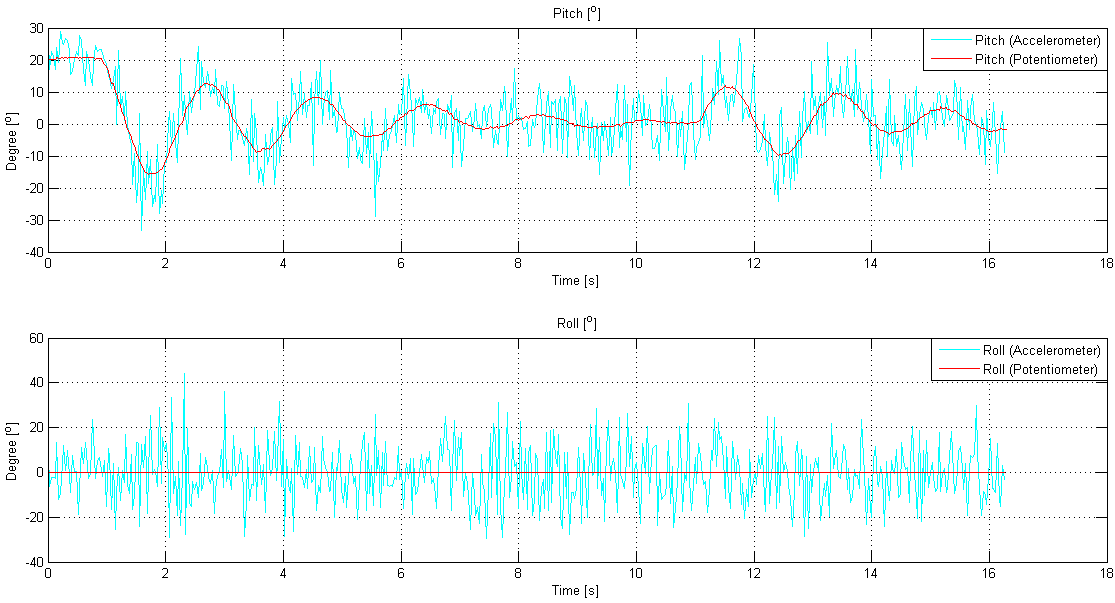
\includegraphics[width =0.7 \paperwidth]{\DocRoot/images/Cyan_unfilter_pitch_and_roll}
	\caption{Unfiltered Accelerometer Output vs Actual Angle}
	\label{Fig:Cyan_unfilter_pitch_and_roll}
\end{figure}
